\documentclass[a4paper,12pt,abstracton]{scrartcl}
\usepackage[utf8]{inputenc}
\usepackage{float}
\usepackage{tikz}
\usepackage{amsmath}
\usepackage{amssymb}
\usepackage{pifont}% http://ctan.org/pkg/pifont
\usepackage[font=small,labelfont=bf]{caption}
\usepackage{graphicx}
%\usepackage{dirtytalk}
\usepackage{multicol}
\usepackage{booktabs}
\usepackage{colortbl}
\usepackage{appendix}
\usepackage{nomencl}
\usepackage{lmodern}
\usepackage[nottoc]{tocbibind}
\usepackage{xcolor}
%\graphicspath{images/}
\usepackage[margin = 3cm]{geometry}
\usepackage{ragged2e} % good alignment
\usepackage{hyperref}
\usepackage{siunitx} % Provides the \SI{}{} and \si{} command for typesetting SI units
\hypersetup{colorlinks=true,
    linkcolor=blue,
    filecolor=magenta,      
    urlcolor=cyan, 
    citecolor=gray}

%\DeclareGraphicsExtensions{.png,.pdf} % low-res (work in progress)
%\DeclareGraphicsExtensions{.pdf,.png}  % high-res (final draft)
%\setlength\parindent{0pt} % Removes all indentation from paragraphs
%\bibliographystyle{unstr}
\setlength\parindent{0pt}
\setlength{\parskip}{0.3em}
\newcommand{\xmark}{\ding{55}}

\renewcommand{\nomname}{List of Symbols}
\renewcommand{\nompreamble}{The following list explains the symbols used within the body of the report.}

\usepackage{etoolbox}
\renewcommand\nomgroup[1]{%
  \item[\bfseries
  \ifstrequal{#1}{E}{Experimental Equipment}{%
  \ifstrequal{#1}{C}{Computational Methods}{%
  \ifstrequal{#1}{T}{Theoretical Concepts}{
  \ifstrequal{#1}{P}{Physical Constants}{}}}}%
]}


\subject{CMP Lab Report} % Matter Physics, Physics, Chemical Physics ?
\title{Zeeman Effect}
\author{Group B9\footnote{Pietro Monticone , Claudio Moroni , Alberto Mosso , Riccardo Valperga.}}

\renewcommand{\listfigurename}{Plots}
\renewcommand{\listtablename}{Tables}
\renewcommand{\nomname}{Nomenclature}


\begin{document}

\section{Normal Zeeman Effect}
\subsection{Longitudinal Configuration}
Here we report the data collected in normal longitudinal configuration:
\begin{table}[H]
\centering
\resizebox{12cm}{!}{
\begin{tabular}{cccccc}
\toprule
I & $\sigma_I$ & B & $\sigma_B$ & $\langle \frac{\delta}{\Delta} \rangle$ & $\sigma_{\langle \frac{\delta}{\Delta} \rangle}$\\
\midrule
\rowcolor{gray!6}  2.685 & 0.02 & 0.188 & 0.002 & 0.070 & 0.002\\
4.840 & 0.02 & 0.333 & 0.002 & 0.140 & 0.003\\
\rowcolor{gray!6}  5.905 & 0.02 & 0.404 & 0.002 & 0.165 & 0.002\\
6.930 & 0.03 & 0.473 & 0.002 & 0.192 & 0.002\\
\rowcolor{gray!6}  7.225 & 0.02 & 0.500 & 0.009 & 0.202 & 0.010\\
\addlinespace
7.855 & 0.02 & 0.539 & 0.009 & 0.218 & 0.002\\
\rowcolor{gray!6}  8.825 & 0.02 & 0.592 & 0.010 & 0.237 & 0.006\\
9.800 & 0.02 & 0.636 & 0.011 & 0.263 & 0.009\\
\bottomrule
\end{tabular}}
\end{table}
\begin{figure}[H]
\hspace{-0.5cm}
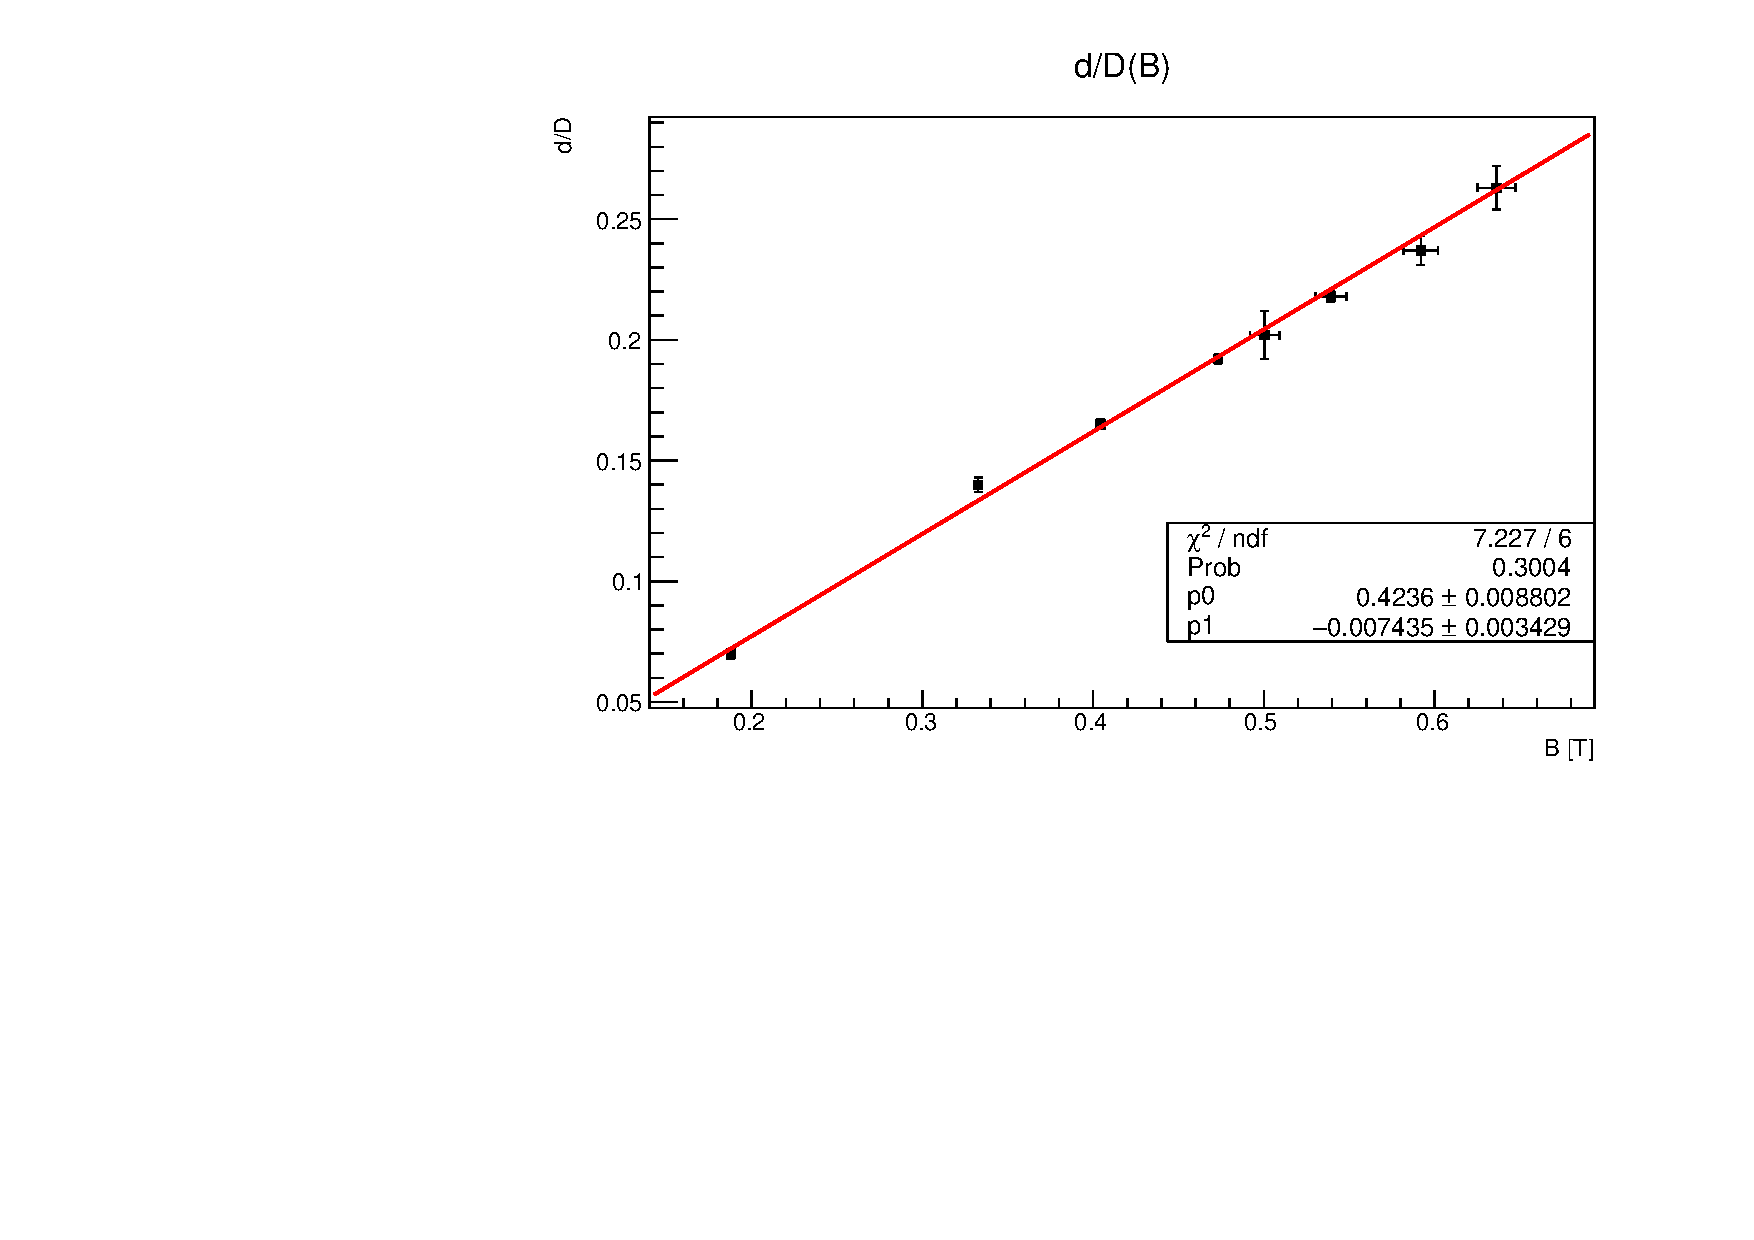
\includegraphics[scale=0.8]{znl.pdf}
\end{figure}
This experiment gives:
\begin{equation*}
\mu_B=(9.7 \pm 0.8868062 )\times 10^{-24} \frac{J}{T}
\end{equation*}
\newpage
%\bibliographystyle{unsrt}
%\bibliography{biblio}
\end{document}
